% !TeX root = ../main.tex

\chapter{硬件加速架构设计}
\section{硬件加速架构的搜索空间}\label{sec:search_space_design}
如第一章第\ref{facing_problems}节所述,在大型数据集的情形,我们从时间复杂度的角度出发,可以考虑的算法只能有堆排序、归并排序、快速排序以及基数排序。所以我们的硬件加速架构的搜索空间,也应该是基于这些算法来进行设计的。

在时间复杂度的同时,我们还需要考虑到各个算法的硬件友好程度。在这四种算法当中:堆排序可以被视为一种分治算法,它可以将一个大的输入序列分成多个较小的子序列并分别排序,最后将这些子序列合并成一个有序序列。这使得堆排序很容易被并行化,不同的处理单元可以同时对不同的子序列进行排序,而后将它们合并在一起;归并排序的并行化也易于实现。它将一个大的输入序列分成多个较小的子序列,并对这些子序列分别进行排序,然后将它们合并在一起。这种特性使得其能够很容易的被并行处理;基数排序是一种非比较排序算法,每次循环中根据元素在每个位上的值来进行排序,这个过程是完全独立的,可以并行执行,因此具有很高的硬件友好度;而对快速排序而言,由于其本质上是基于比较的算法,涉及到大量的非相邻元素的比较和交换,而为了进行比较和交换操作,需要访问数组中的随机元素,而这种随机访问在硬件中需要通过内存地址映射或多级缓存等技术来实现,增加了设计的复杂性和开销。此外,快速排序的递归结构也不利于在硬件中实现,因为递归需要消耗大量的存储器和控制器资源。而与此相对的,堆排序、归并排序和基数排序则都具有很好的局部性,即访存序列元素的时,可以访问一段连续的存储块,因此他们属于硬件友好型的算法,更加利于硬件加速。

基于上述的分析和讨论,我们的搜索空间当中只包含了归并排序、堆排序以及快速排序。但是这并不意味着硬件搜索空间中仅仅包含了三种选项:由于归并排序的特殊性,理论上来说,我们只需要生成多个小的有序序列,也可以通过之前所说的k路归并排序的方式进行排序;同时,基数排序根据进制的不同,也可以分为2进制、8进制、16进制的基数排序。我们的硬件架构搜索空间如表\ref{table:search_space}所示,一共13个备选方案。

\begin{table}[htbp]
\centering
\caption{硬件架构搜索空间}
\resizebox{\linewidth}{!}{
\begin{tabular}{ccc}
\toprule
\multicolumn{2}{c}{混合算法}         & 单一算法     \\
\midrule
2进制基数排序+传统k路归并  & 2进制基数排序+败者树归并  & 归并排序     \\
8进制基数排序+传统k路归并  & 8进制基数排序+败者树归并  & 2进制基数排序  \\
16进制基数排序+传统k路归并 & 16进制基数排序+败者树归并 & 8进制基数排序  \\
堆排序+传统k路归并      & 堆排序+败者树归并      & 16进制基数排序 \\
                &                & 堆排序      \\
\bottomrule
\end{tabular}}
\label{table:search_space}
\end{table}


\section{硬件加速架构的设计}

根据第\ref{sec:search_space_design}节所阐述的搜索空间,我们可以发现我们的硬件架构可以由几个模块构成:基数排序模块、归并排序模块、堆排序模块,以及一些IO控制模块等。将这些模块进行组合,即可组成上述硬件架构搜索空间中的各种架构,实现对其性能的评估。
\subsection{基数排序模块设计}
\subsubsection{传统基数排序算法在HLS实现中面临的问题}
对于传统的排序算法来说,在每一个循环中,我们按照每个数对应数位的值将其放入到“桶”中,再按照顺序将其取出,作为新的待排序数组。在取出过程中,要保证每个“桶”中的数取完之后就开始从下一个桶中取数,我们需要给每一个桶分配一个指针:每输入一个数指针的值加1,每输出一个数指针的值减1,当指针的值为0时,则说明该桶中的数已经全部取出,基本算法如图\ref{fig:traditional_radix_sort}所示:
\begin{figure}[htbp]
    \centering
    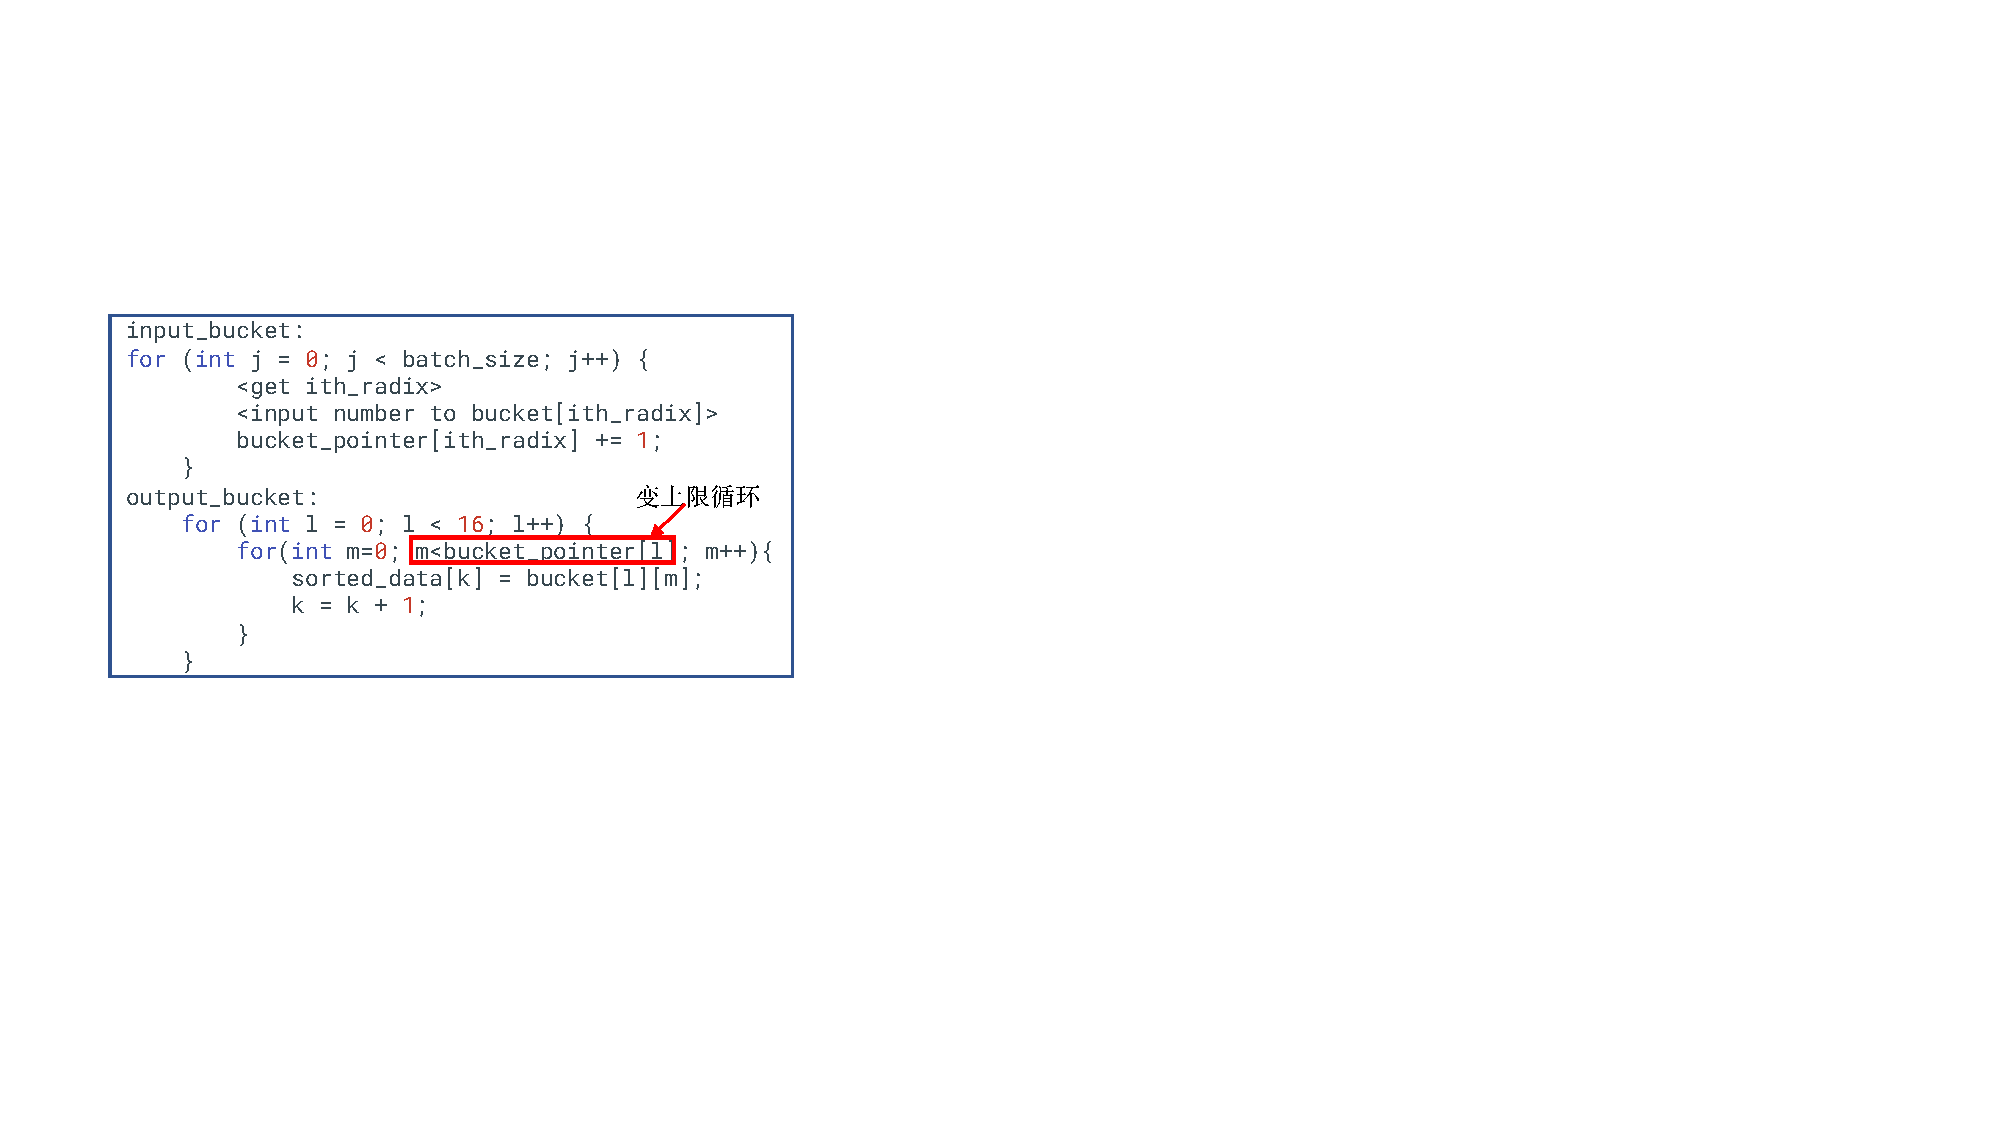
\includegraphics[width=12cm]{figures/traditional_radix_sort_algorithm.pdf}
    \caption{传统基数排序算法示意。红圈标出的即为变上限循环}
    \label{fig:traditional_radix_sort}
\end{figure}

然而,在这个过程中,会存在着若干问题,从而影响到硬件的执行效率:
\begin{enumerate}
    \item 为了考虑最坏情况(所有数的第n位数都是一样的),每一个“桶”的大小都必须和待排序数组大小相同,这就造成了极大的空间浪费,对于BRAM来说,其本身存储空间就较小,当待排序数组增大时,这种资源浪费将急剧增加,让可以排序数组的数量的上限大大降低;
    \item 在“桶”的输出循环当中,由于每个桶的指针值各不相同,所以该循环是一个变上限循环。对于HLS来说,如果使用变上限循环,则无法通过\verb|#pragma HLS pipeline|或者\verb|#pragma HLS dataflow|来实现硬件架构的流水化,这对于提升吞吐率和减低延迟来说是非常不利的;
    \item 由于基数排序算法本身的限制,在“桶”输入和“桶”输出循环当中存在“写后读”的数据相关,而这个循环周期会随着输入数组的增大而增大,当输入数组特别大时,将会造成很长的等待和空转周期。
\end{enumerate}

\subsubsection{对应的优化措施}
\begin{figure}[htbp]
    \centering
    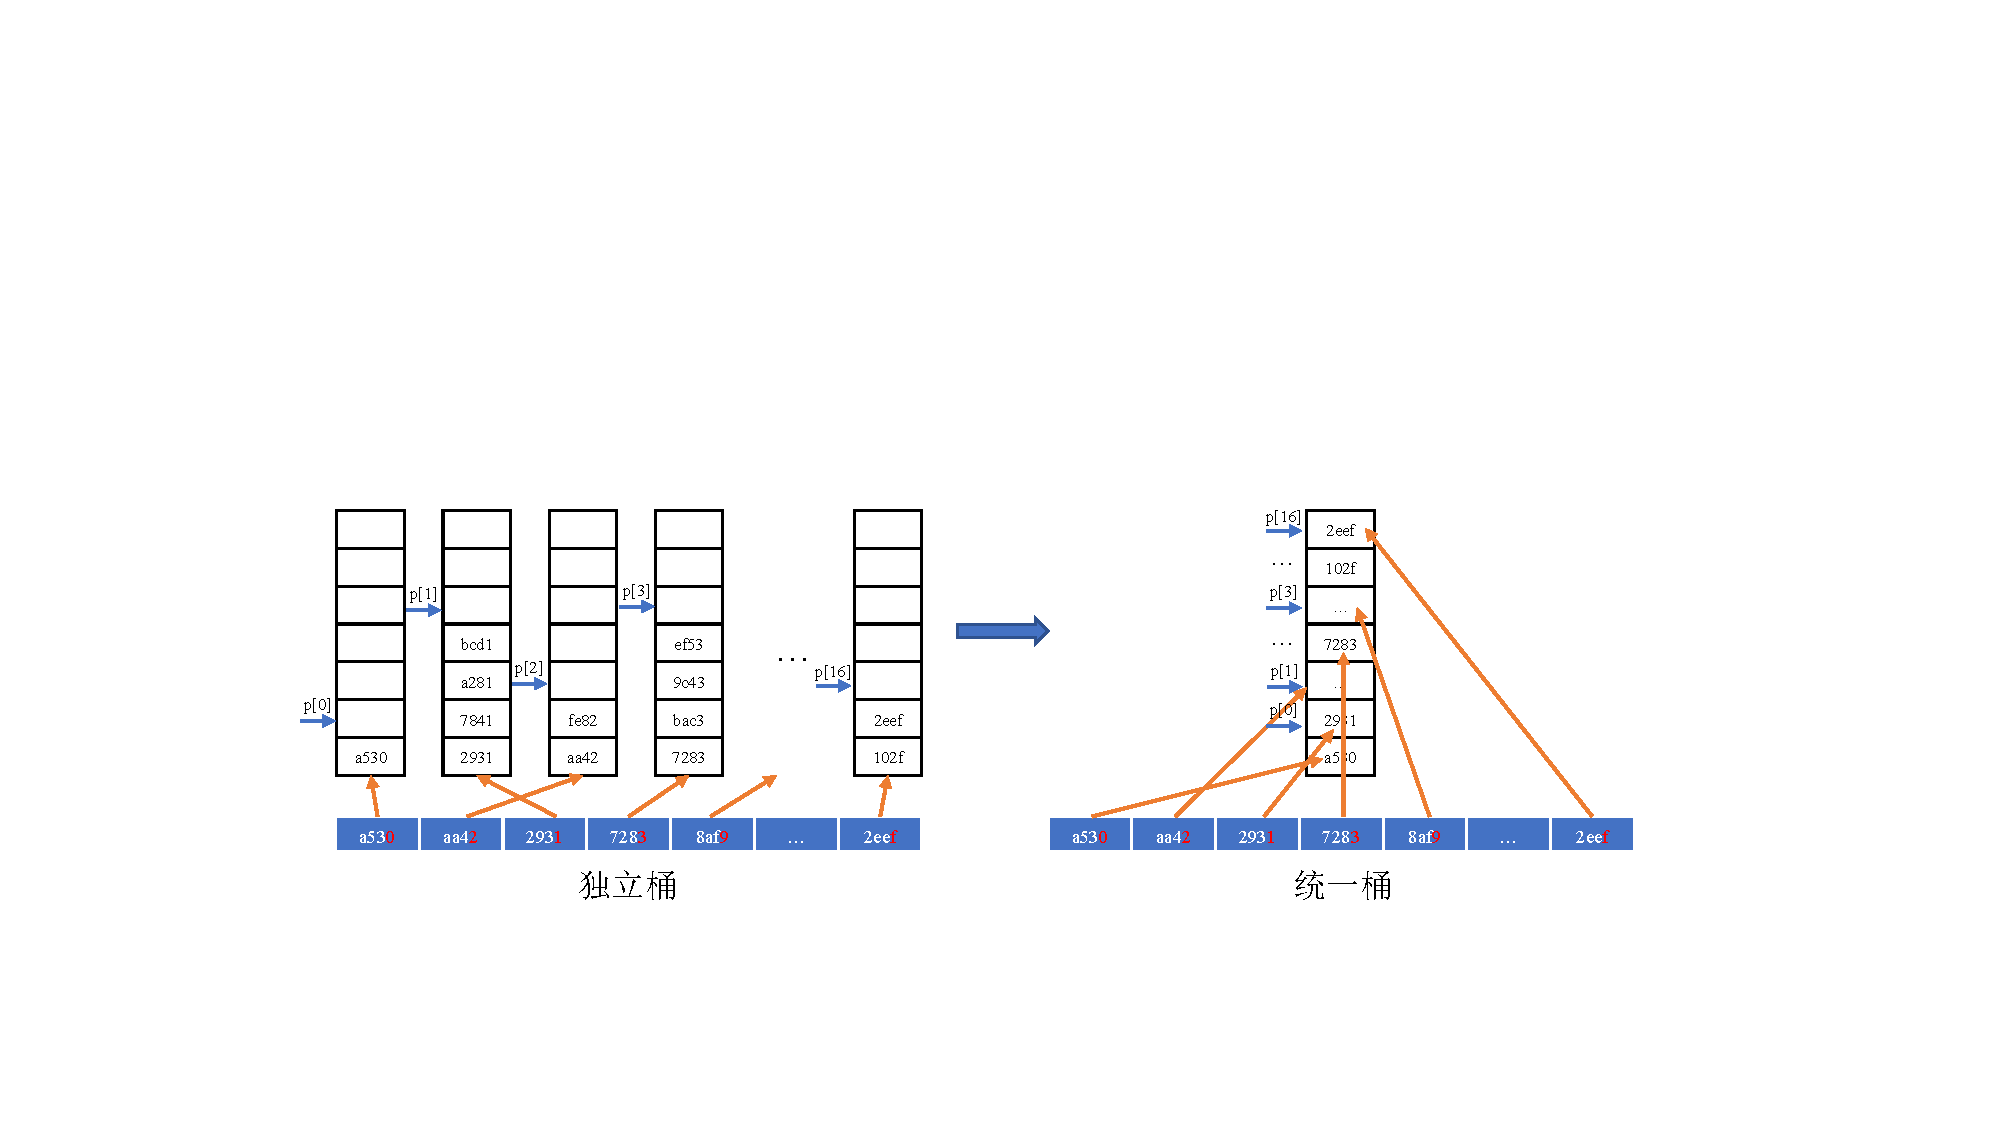
\includegraphics[width=\linewidth]{figures/unified_bucket.pdf}
    \caption{统一桶基数排序示意图}
    \label{fig:unified_bucket}
\end{figure}

\begin{figure}[htbp]
    \centering
    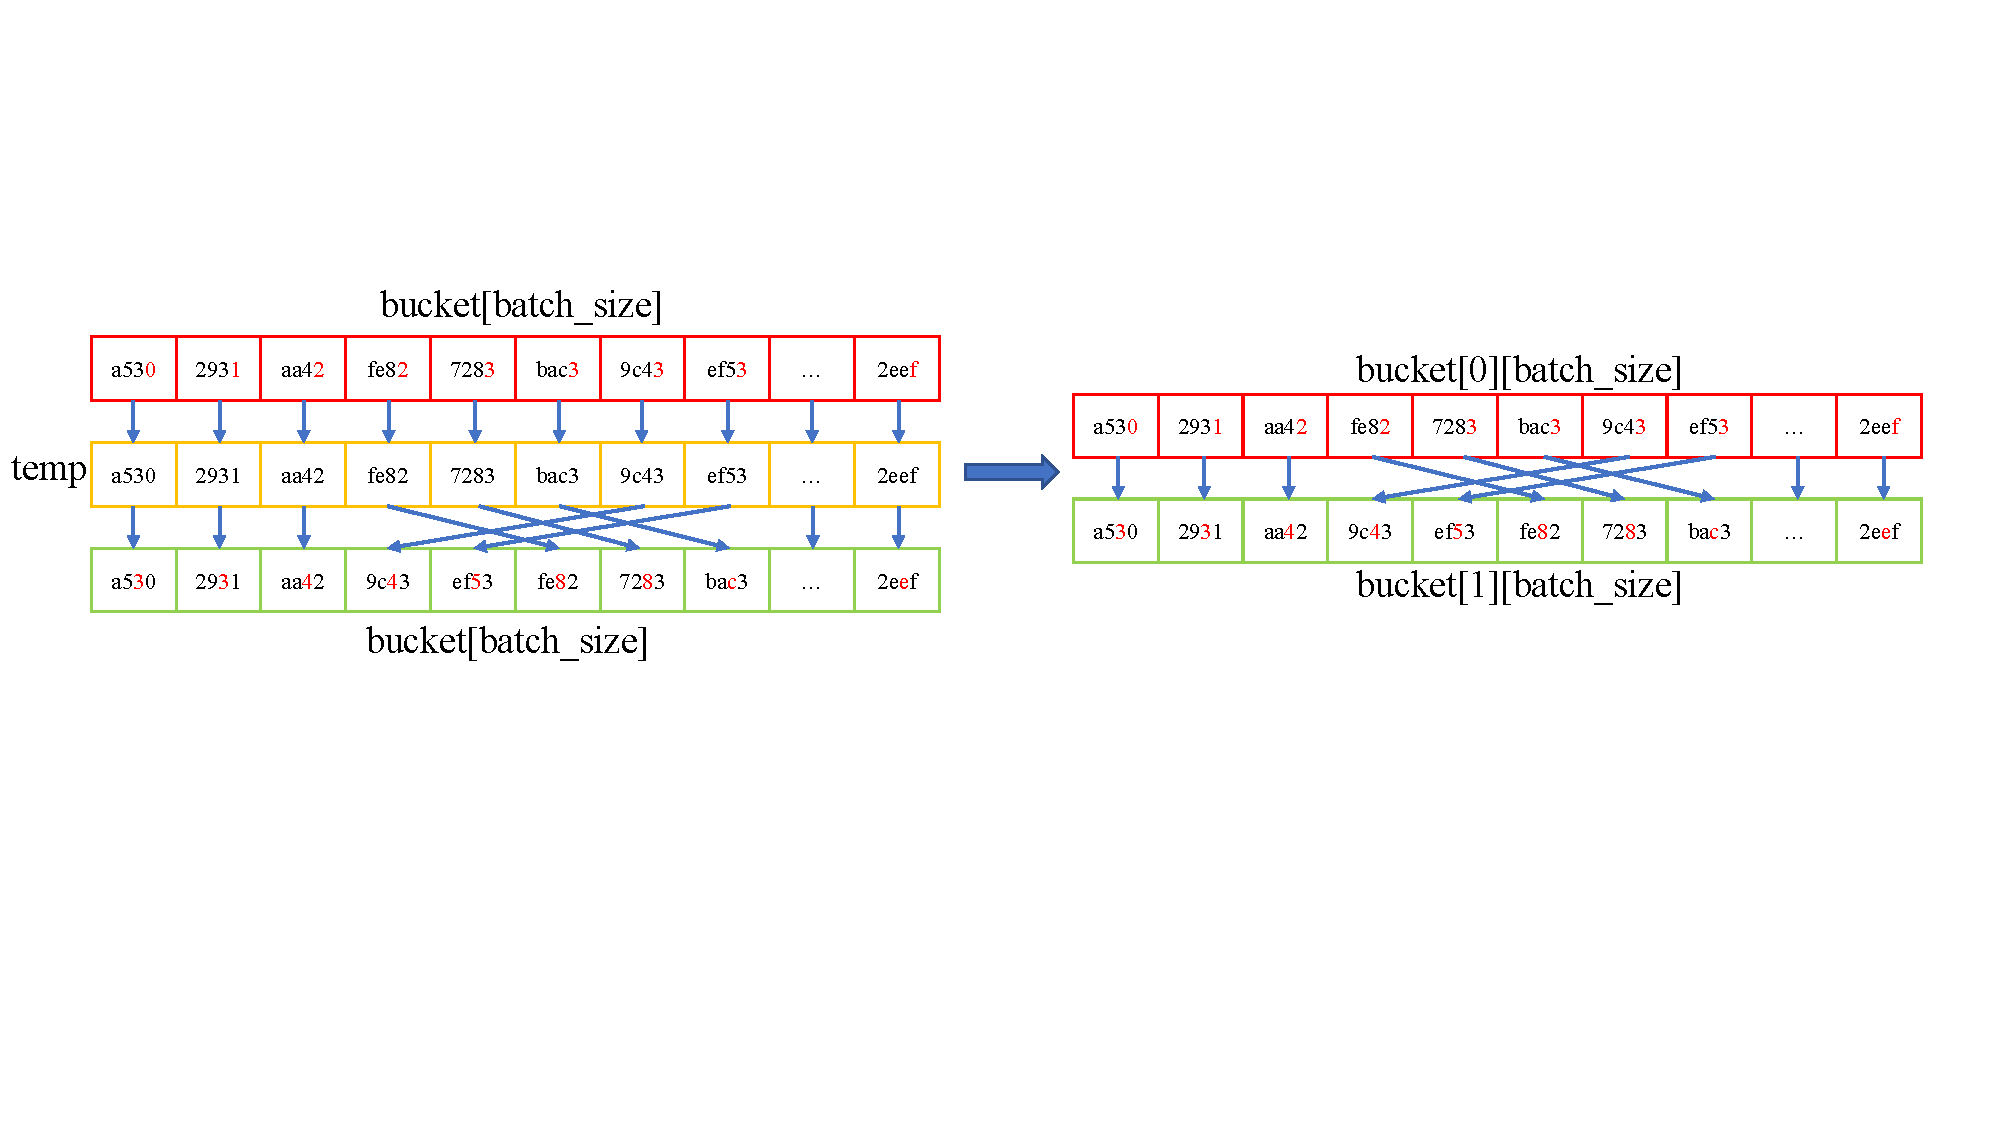
\includegraphics[width=\linewidth]{figures/pingpong_buffer.pdf}
    \caption{Ping-Pong buffer示意图}
    \label{fig:pingpong_buffer}
\end{figure}
针对上述提出的问题,我们创新性的给出如下优化措施:

\begin{enumerate}
    \item 采用统一“桶”的方式,通过多个指针来分隔不同数位值的数。具体而言,如果采用n进制基数排序,则统一“桶”中有$2^n$个指针。通过使用统一“桶”,我们能够大大减少BRAM的使用量,使得片上大数据集排序成为可能。其基本思想如图\ref{fig:unified_bucket}所示。
    \item 在采用统一“桶”方式时,由于我们输出“桶”过程不需要考虑每个部分的指针位置,而是直接将“桶”中元素顺序读出,因此不存在变上限循环,这也使得我们能够通过\verb|#pragma HLS pipeline|实现硬件流水化。
    \item 采用Ping-Pong buffer技术,即设置两个统一“桶”,在一个循环中,一个桶作为输出,一个桶作为输入。具体来说,在奇数循环中,排序模块从0号桶顺序读取数据,根据不同数的基数大小放入到1号桶当中;在该循环的下一个循环当中(即偶数循环),我们直接从1号桶中顺序读取数据,并按照不同数的基数大小放入到0号桶当中。这样做的一个好处是省去了中间数组的写入与读出,而是两个桶直接进行数据的输入和输出,从而大大降低了延迟和数据相关问题,使得硬件架构能够进一步流水化。其基本思想如图\ref{fig:pingpong_buffer}所示。
\end{enumerate}


需要注意的是,我们的基数排序模块是灵活的,可以适用于任意$2^n$进制数的排序。在接下来的实验当中,我们仅考虑常用的2进制、8进制、16进制排序。
\subsection{归并排序模块设计}
\subsubsection{传统归并排序模块设计}
传统归并排序模块相对简单。对于两路有序序列输入,分别比较它们首位元素,将较小者选出放入输出序列当中,并将指针向后移位,最后重复上面的操作。需要注意的是,在最后需要判断数组元素是否已经排空,如果已经排空而另外一个数组仍有数,则将另外数组中的数有序输出即可。
\subsubsection{单一归并排序模块设计}
\begin{figure}[htbp]
    \centering
    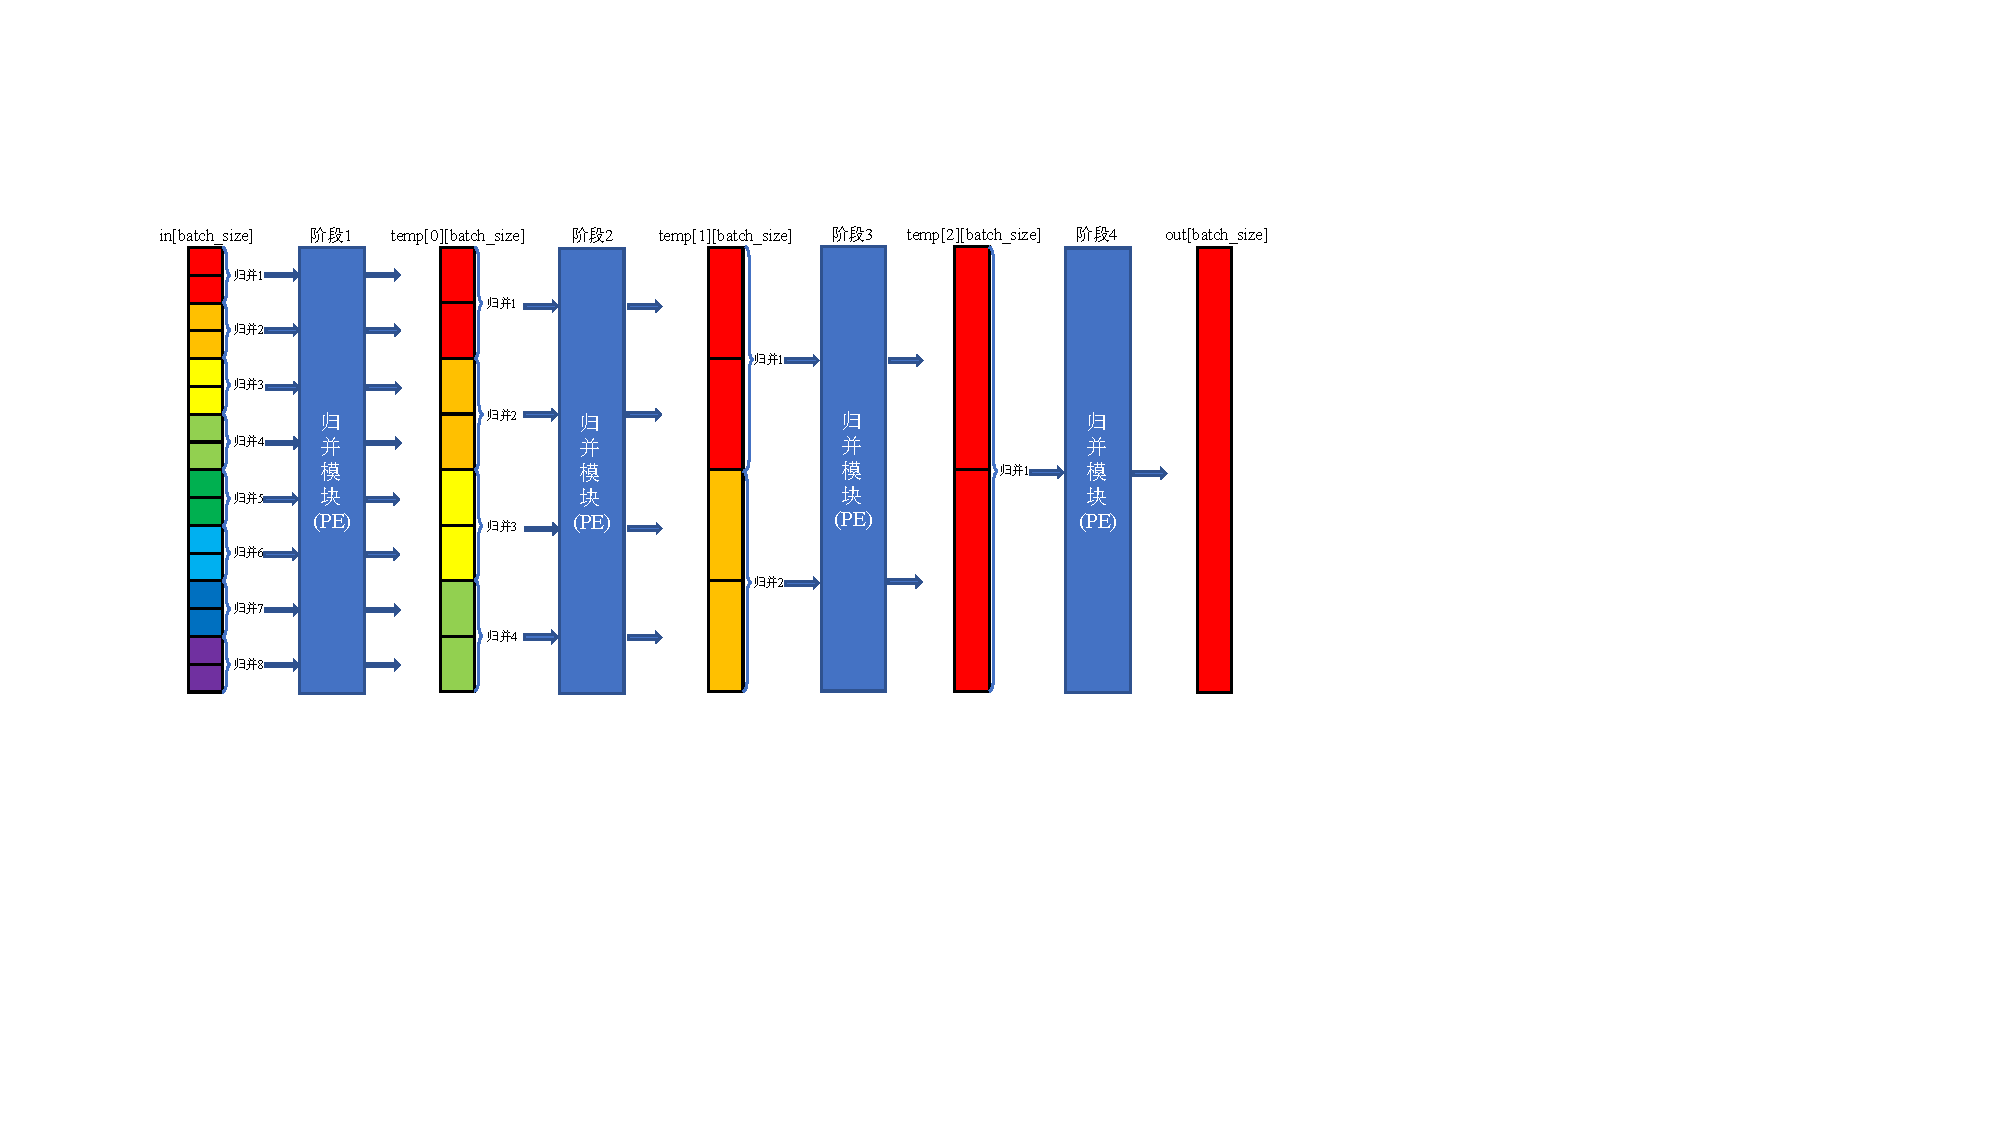
\includegraphics[width=\linewidth]{figures/merge_sort.pdf}
    \caption{单一归并排序算法示意}
    \label{fig:merge_sort}
\end{figure}
如果我们想通过单一的归并排序模块来实现对一个无序序列的排序,我们还需要对归并排序模块进行修改以适应硬件特性。单一归并排序可以理解为首先将数组分割成多个长度为2的小块,分别对它们两两归并,然后增加步长到4,再进行两两归并,最后不断重复的过程。如图\ref{fig:merge_sort}所示。但是不同于二输入归并模块,在单一归并模块中,我们只有一个输入,并存放在BRAM当中。由于BRAM最多只能允许同时两路访问,所以并不能完全并行化。因此我们尝试在每个阶段内部实现排序流水线,同时在不同阶段中间应用\verb|#pragma HLS dataflow|。在实例化暂存数组\verb|temp|时,采用\verb|#pragma HLS array_partition|对其进行分割,将其实例成多个BRAM块,从而实现并行访问。这样下来,在综合的时候,硬件能够达到II=1的流水线,性能得到极大的提升。

\subsubsection{败者树归并模块设计}

败者树算法的主要思想如图\ref{fig:loser_tree}所示。通过HLS编写算法时,由于其涉及到数据交换的操作,我们可以将败者树中的元素定义一个新的数据结构Item,里面包含了该元素所在的败者树位置以及元素数值的大小。同时,在循环中,我们可以插入\verb|#pragma HLS pipeline|来将其流水线化,从而达到降低延迟、提升性能的目的。在进行败者树归并的时候,我们需要注意在后期可能会有部分输入数组已经归并完成的情况,这个时候我们需要判断数组指针是否已经超过batch\_size,如果超过的话,则将该叶子结点设为int数据类型能够表达的最大值(2147483647),从而确保其不会参与到败者树归并过程当中。
\subsection{堆排序模块设计}
堆排序模块主要分为三个部分:构建大顶堆、交换/推出元素、重构大顶堆。我们可以分别定义交换元素函数swap,构建大顶堆函数maxHeapify;在重构操作中,可以复用构建大顶堆函数。需要注意的是,HLS对于递归定义的函数的支持十分有限,而堆排序在一般的软件算法中,常采用递归定义的方式。因此,在写HLS代码时,我们应该避免采用递归定义:如在定义构建大顶堆函数时,我们可以让循环一直持续,直到根元素为最大元素,即为构建完成。同时,在循环当中,我们也利用了循环展开以及流水线的措施,实现了II=1的流水线结构。

\subsection{混合排序算法设计}


混合排序算法的主要模式分为两种:多路排序+传统k路归并排序、多路排序+败者树归并排序。这里的多路排序,可以是n进制基数排序或者堆排序。其基本思想如图\ref{fig:k_way_sorting}所示。对于多路归并排序来说,k的值可以自由选择。综合考虑硬件资源、数据集大小等因素,我们统一设定k=64。
%如果时间来得及可以介绍一下为啥k=64是最优选项。
多路排序算法的并行度可以通过Vitis HLS中的schedule viewer直观的看出来。以64路基数排序+多路归并排序为例,图\ref{fig:schedule_viewer}展示的即为其在各个阶段的任务执行情况。可见在第一个时钟周期,64路基数排序实现了并行执行;接下来的时钟周期均实现了并行的归并排序,可见其成功实现了算法的并行化。


\begin{figure}[htbp]
    \centering
    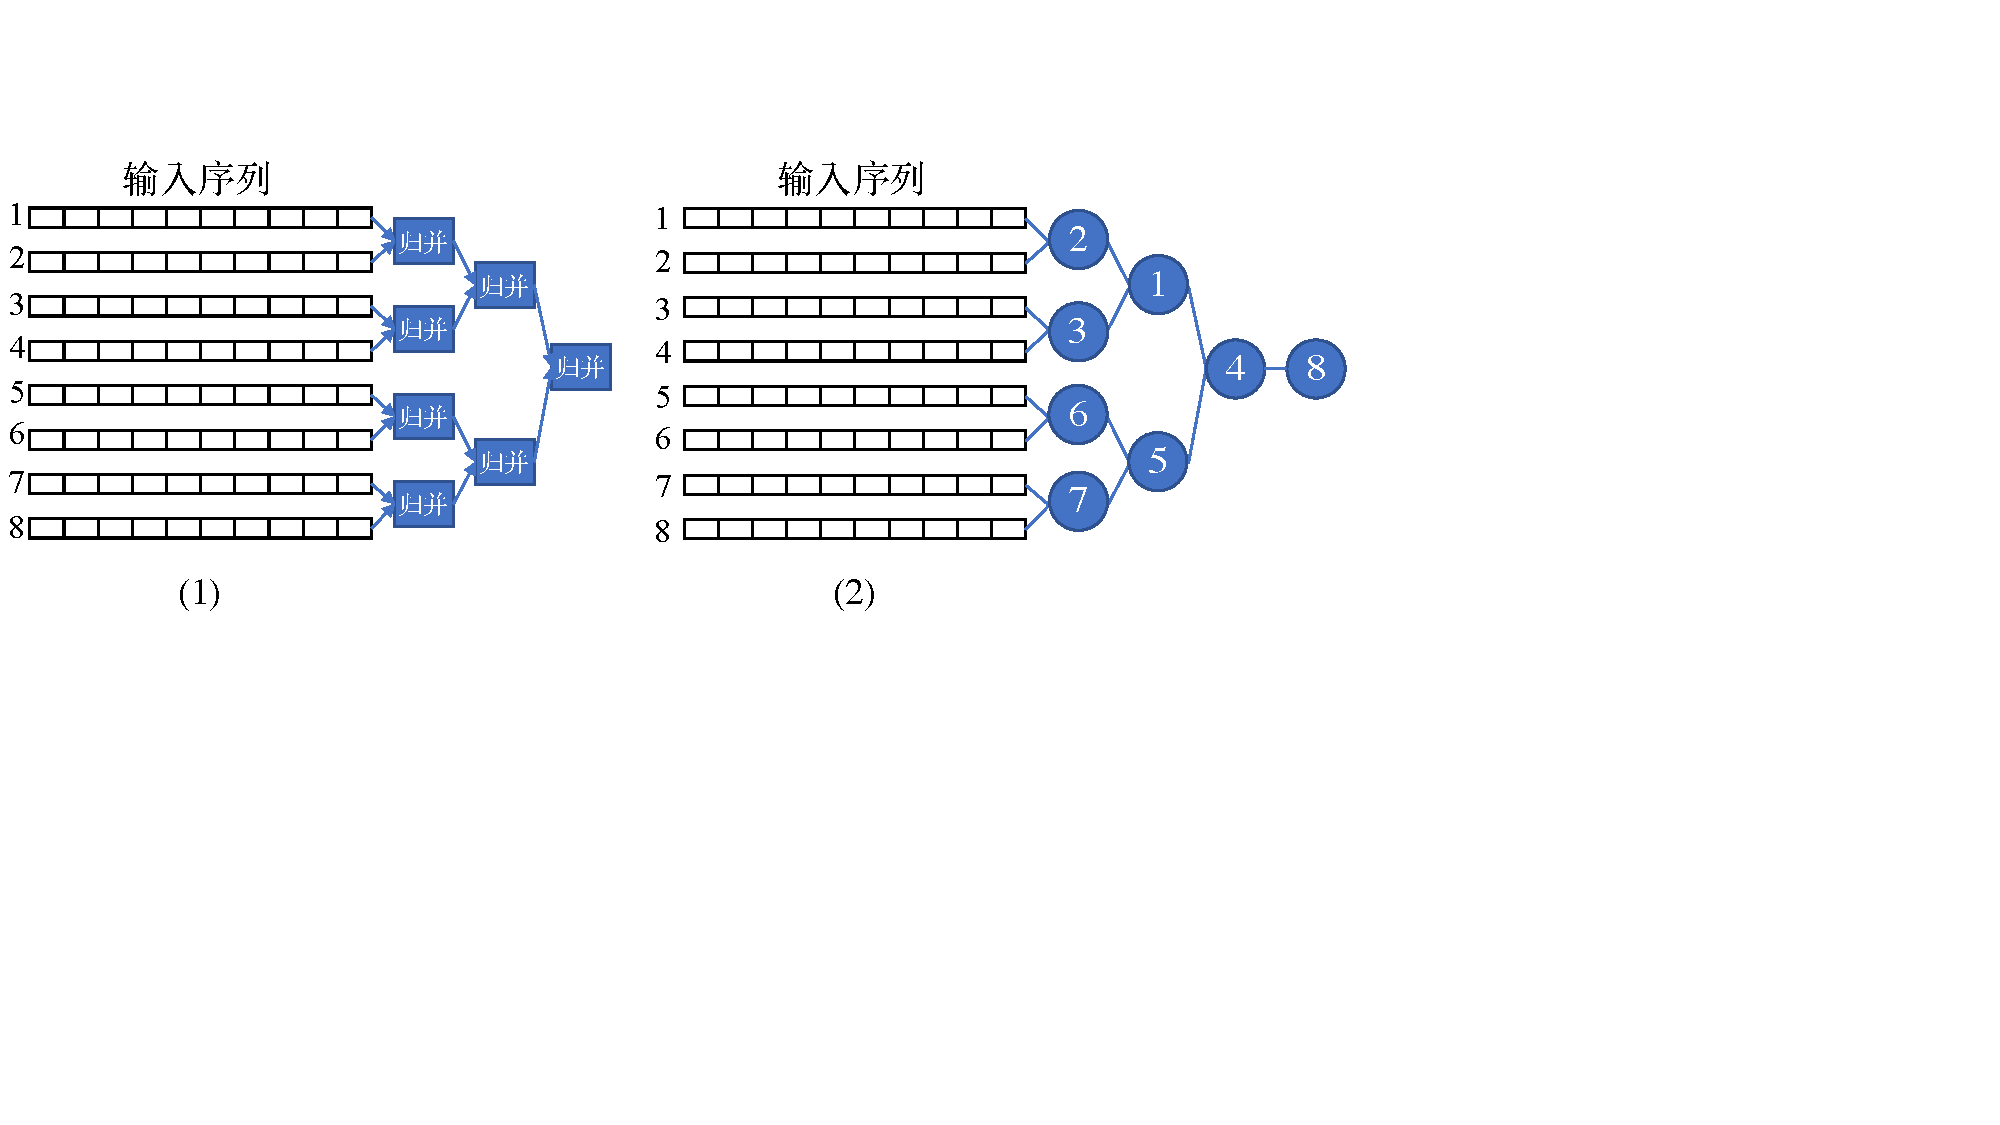
\includegraphics[width=\linewidth]{figures/k_way_sorting.pdf}
    \caption{混合算法排序示意图。(1) 多路排序+传统k路归并排序;(2) 多路排序+败者树归并排序}
    \label{fig:k_way_sorting}
\end{figure}


\begin{figure}[htbp]
    \centering
    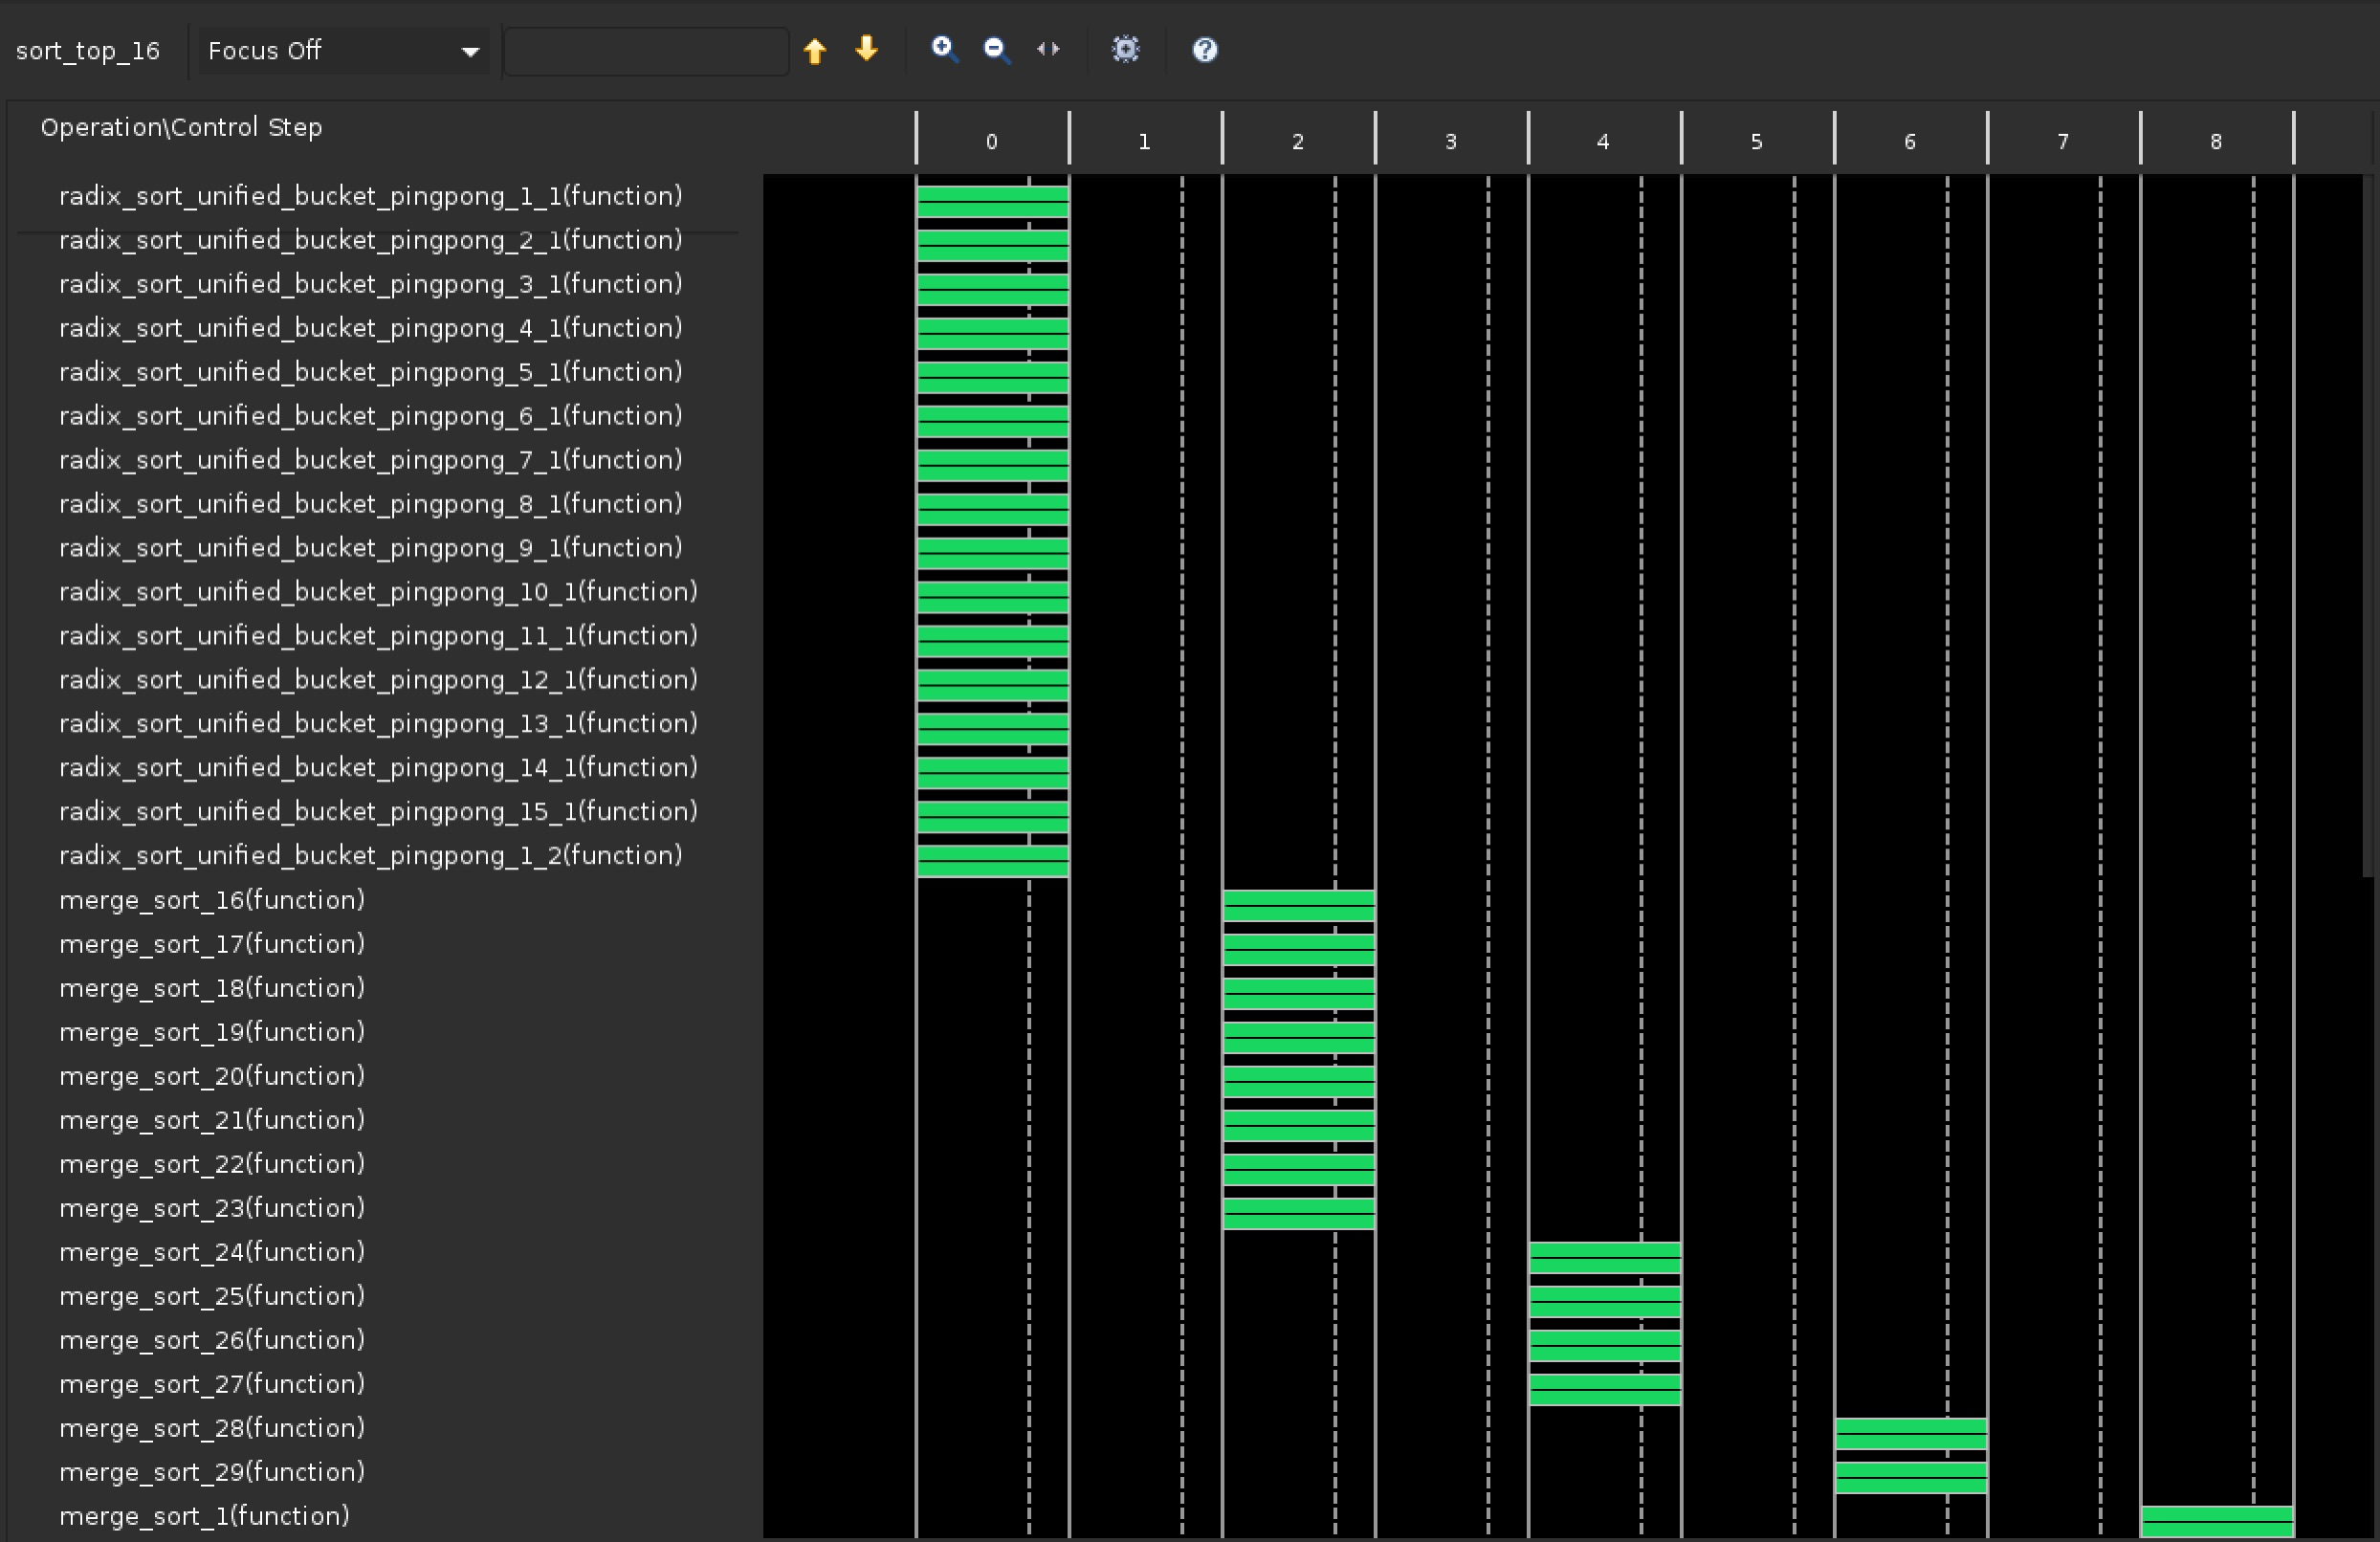
\includegraphics[width=\linewidth]{figures/schedule_viewer.jpeg}
    \caption{Vitis HLS Schedule Viewer界面}
    \label{fig:schedule_viewer}
\end{figure}


